\section{Motivation}

\begin{frame}\frametitle{Tetrapod of Knowledge}
\begin{itemize}
\item Narration: informal-but-rigorous math
\item Deduction: logic and type systems
\item Computation: algorithms
\item Data: tables for large sets and functions
\item Representation: content dictionaries, ontologies
 \lec{essential for inter-operability}
\end{itemize}

\begin{center}
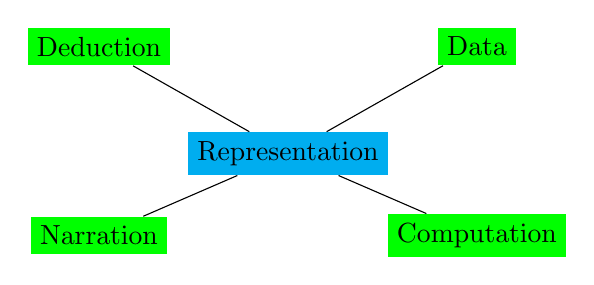
\begin{tikzpicture}[scale=.8]
\node[fill=green] (D)  at (-3,3)   {Deduction};
\node[fill=green] (T)  at (3,3)    {Data};
\node[fill=green] (Cm)  at (3,0)   {Computation};
\node[fill=green] (N)  at (-3,0)   {Narration};

\node[fill=cyan] (Cn)  at (0,1.3)   {Representation};
\draw[-] (Cn) -- (D);
\draw[-] (Cn) -- (T);
\draw[-] (Cn) -- (Cm);
\draw[-] (Cn) -- (N);
\end{tikzpicture}
\end{center}
\end{frame}

\begin{frame}\frametitle{MMT as a System Integration Platform}
All system interfaces formalized in MMT \\
$\to$ semantics-aware tool integration while maintaining existing work flows
\begin{center}
\begin{tikzpicture}[xscale=1.5]
\tikzstyle{conn}=[angle 45-angle 45]
\tikzstyle{field}=[draw,rectangle]

\node[field] (KM) at (0,2.8)  {Data, tables};
\node[field] (Spec) at (0,-2.8)  {Narration, documents};
\node[field,rotate=-90] (Spec) at (3.7,0)  {Computation, programs};
\node[field,rotate=90] (Ded) at (-3.3,0)  {Deduction, proofs};

\node[draw,ellipse] (U) at (0,0)  {MMT as Mediator};
\node (Sp) at (1,-2)  {WWW};
\node (TP) at (-2,-1)  {Specification};
\node (PA1) at (-2,.7)  {Provers};
\node (PA2) at (-2,1.3)  {Model checkers};
\node (CAS) at (2.5,.5)  {Symbolic comp.};
\node (Op) at (2,1.3)  {Numeric comp.};
\node (Sa) at (2,-.7)  {Progr. lang.};
\node (Sc) at (2,-1.3)  {Program synthesis};
\node (M) at (-1,2)  {Math databases};
\node (MWS) at (1,2)  {Query Languages};

\only<2>{\begin{scope}[red]}
\node (He) at (-1,-2)  {\LaTeX};
\draw[conn](U) -- (He);
\node (tt) at (-2,-2) {this talk};
\only<2>{\end{scope}}

\draw[conn](U) -- (Sp);
\draw[conn](U) -- (M);
\draw[conn](U) -- (MWS);
\draw[conn](U) -- (Op);
\draw[conn](U) -- (CAS);
\draw[conn](U) -- (Sa);
\draw[conn](U) -- (Sc);
\draw[conn](U) -- (TP);
\draw[conn](U) -- (PA1);
\draw[conn](U) -- (PA2);
\end{tikzpicture}
\end{center}
\end{frame}

\section{Design}

\begin{frame}\frametitle{Ideal System}
\begin{blockitems}{Requirements}
\item Authors can mix (at least) MMT and LaTeX in the same file
 \begin{itemize}
 \item multiple nesting levels
 \item top level can be either format
 \end{itemize}
\item Control passes between MMT and LaTeX processor
 \begin{itemize}
 \item sharing the same context
 \item communicating context changes
 \end{itemize}
\item Produces OMDoc, pdf, HTML, etc.
\end{blockitems}

\begin{blockitems}{Problems}
\item No way to get LaTeX processor to interact dynamically with other systems
\item No way to write a new LaTeX processor for the occasion
\end{blockitems}
\end{frame}

\begin{frame}\frametitle{Realistic Options}
\begin{blockitems}{Symmetric}
\item new document format with alternating/nested MMT and LaTeX chunks
\item generate \texttt{.tex} and \texttt{.mmt} files, process separately, merge the outputs
\end{blockitems}
\lec{failed 2016 CICM submission, difficult but still interesting}

\begin{blockitems}{MMT-led}
\item .mmt file with interspersed LaTeX chunks
\item MMT generates \texttt{.tex} file
\end{blockitems}
\lec{future work}

\begin{blockitems}{LaTeX-led}
\item .tex file with interspersed MMT chunks
\item LaTeX generates \texttt{.mmt} file
\end{blockitems}
\lec{\color{red}this talk}
\end{frame}

\begin{frame}\frametitle{Work flow}
BibTeX model:
\begin{center}
\begin{tabular}{|l||l|l|l|}
\hline
& Input & Processor & Output \\
\hline
\hline
Step 1 & \texttt{d.tex} & LaTeX & \texttt{d.pdf} \\
       &                &       & \texttt{d.tex.mmt}\\
\hline
Step 2 & \texttt{d.tex.mmt} & MMT & \texttt{d.tex.omdoc} \\
       &                    &     & \texttt{d.tex.sty}\\
\hline
Step 3 & \multicolumn{3}{c|}{Run LaTeX again} \\
\hline
\end{tabular}
\end{center}

2 components:
\begin{itemize}
\item \texttt{mmttex.sty} package for LaTeX
 \begin{itemize}
 \item Step 1: writes out MMT chunks to \texttt{d.tex.mmt}
 \item Step 3: replaces MMT chunks with code from \texttt{d.tex.sty}
 \end{itemize}
\item \texttt{latex-mmt} plugin for MMT
 \begin{itemize}
 \item Step 2: processes \texttt{d.tex.mmt}, generates \texttt{d.tex.sty}
 \item once at beginning: generates \texttt{.sty} files for any other MMT content
 \end{itemize}
\end{itemize}

\end{frame}

\begin{frame}\frametitle{Easy to Integrate with Existing Work Flows}
 \begin{blockitems}{One extra LaTeX package}
 \item no conflicts with other packages
 \item no dependency on LaTeX editor
 \end{blockitems}

 \begin{blockitems}{One extra shell command}
 \item run MMT as black box
 \item easy to integrate with makefiles, editor shortcuts
 \end{blockitems}

 \begin{blockitems}{Documents re-compilable without MMT}
 \item just include \texttt{d.tex.sty} when uploading sources
 \item running LaTeX still produces \texttt{d.tex.mmt} but it has no effect
  \lec{needed for academic publication}
 \end{blockitems}

\end{frame}

\begin{frame}\frametitle{Enables Semantic Formulas inside LaTeX}
\begin{blockitems}{Semantics processing of \texttt{.tex} files}
\item MMT parsing and type-checking during LaTeX compilation
 \lec{semantic errors produce LaTeX errors}
\item formulas enriched with inferred information
 \lec{implicit arguments, omitted types}
\end{blockitems}

\begin{blockitems}{Semantically enriched formulas in \texttt{.pdf}}
\item tooltips with variable types
\item hyperlinks from symbol usage to definition
\item whatever else we can get the pdf viewers to support
 \lec{e.g., pdf JavaScript exists but barely supported}
\end{blockitems}
\end{frame}

\section{Example and Demo}

\begin{frame}\frametitle{3 kinds of MMT content}
\begin{center}
\begin{tabular}{|l||l|l|l|}
\hline
Kind & defined in & function \\
\hline
\hline
Pres.-rel. chunks   & \multirow{2}{*}{LaTeX document}  & payload\\
\cline{1-1}\cline{3-3}
Pres.-irrel. chunks &  & \multirow{2}{*}{needed by payload}\\
\cline{1-2}
Backgr. Knowledge         & elsewhere & \\
\hline
\end{tabular}
\end{center}

\begin{itemize}
\item Presentation-\textbf{relevant} MMT chunks
 \begin{itemize}
 \item formulas written in MMT syntax, processed by MMT
 \item produce semantically enriched formulas in the \texttt{.pdf} file
 \end{itemize}
 \lec{e.g., $2+x$}
\item Presentation-\textbf{irrelevant} MMT chunks
 \begin{itemize}
 \item provide context for the pres.-rel. chunks
 \item part of \texttt{.tex} file
 \item no effect on \texttt{.pdf} file
 \end{itemize}
  \lec{e.g., type of $x$}
\item Background knowledge
 \begin{itemize}
 \item available in MMT independent of LaTeX document
 \item define formal language(s) used in \texttt{tex} file
 \end{itemize}
 \lec{e.g., definition of $+$}
\end{itemize}
\end{frame}

\begin{frame}\frametitle{Game Plan}
\begin{itemize}
\item Background knowledge: typed first-order logic in MMT
\item Write a LaTeX document using MMTTeX
 \lec{these slides themselves!}
 \begin{enumerate}
  \item define theory of groups
  \begin{itemize}
   \item informally as usual
   \item additional pres.-irrel. chunks for formalization
  \end{itemize}
  \item write formulas about groups in formal MMT syntax
 \end{enumerate}
\end{itemize}
\end{frame}

